\documentclass[aspectratio=169]{beamer}

\title{On Elementary Properties of a Multidimensional Generalization of the Euclidean Algorithm}
\author{Daniel Knaack}
\date{July 1, 2025}

\usepackage{tikz}
\usepackage{fontspec}
\usepackage{unicode-math}
\usepackage{standalone}
\usepackage{adjustbox}
\usepackage{emoji}

\usetikzlibrary{
  decorations.pathreplacing,
  calligraphy,
  intersections,
  backgrounds,
  graphdrawing,
  graphs,
  calc,
  matrix,
  3d,
  positioning
}

\tikzset{>=stealth}
\newtheorem{conjecture}{Conjecture}
\newcommand\floor[1]{\left\lfloor#1\right\rfloor}

\usetheme{metropolis}
\usefonttheme[onlymath]{serif}
\setbeamertemplate{caption}{\raggedright\insertcaption\par}
\setmathfont{TeX Gyre Pagella Math}

\begin{document}

\begin{frame}
  \maketitle
\end{frame}

\begin{frame}
  \frametitle{Representation of Real Numbers}
  \begin{columns}[T]
    \column{0.33\textwidth}
    \begin{center}
      \textbf{Rational Numbers} \\
      Decimals
      \[
        \frac{22}{7} = 3.\overline{142857}
      \]
    \end{center}

    \column{0.33\textwidth}
    \begin{center}
      \textbf{Quadratic Irrationals} \\
      Continued Fractions
      \begin{align*}
        \sqrt{2} & = 1 + \cfrac{1}{2 + \cfrac{1}{2 + \cfrac{1}{⋱}}}
      \end{align*}
    \end{center}
    \column{0.33\textwidth}
    \begin{center}
      \textbf{Cubic Irrationals} \\
      ?
      \[\sqrt[3]{5} = ? \vphantom{\cfrac{1}{a₀}}\]
    \end{center}
  \end{columns}
\end{frame}

\begin{frame}
  \begin{problem}[Hermite, 1839]
    Does there exist a representation of the \alert{real numbers as a sequence of integers}
    such that the representation is \alert{eventually periodic} if and only if
    the number is \alert{\alt<2>{an algebraic number of degree $d$}{a cubic irrational}}?
  \end{problem}
\end{frame}

\begin{frame}
  \frametitle{Outline}
  \small
  \begin{columns}
    \column{0.49\textwidth}
    \textbf{Quadratic Irrationals}:
    \begin{enumerate}
      \item The Euclidean Algorithm
      \item Fibonacci Numbers
      \item Continued Fractions
      \item Periodicity and Quadratic Irrationals
    \end{enumerate}

    \column{0.49\textwidth}
    \textbf{Algebraic Numbers}:
    \begin{enumerate}
      \item The Generalized Euclidean Algorithm
      \item Higher-Order Fibonacci Numbers
      \item Multidimensional Continued Fractions
      \item Periodicity and Algebraic Numbers?
    \end{enumerate}
  \end{columns}
\end{frame}

\begin{frame}
  \frametitle{The Euclidean Algorithm}
  \small
  \begin{columns}[T]
    \column{0.45\textwidth}
    \begin{problem}[Greatest Common Divisor]
      \begin{itemize}
        \item \textbf{Input}: $a, b ∈ ℤ$.
        \item \textbf{Output}: $c = \gcd(a, b)$.
      \end{itemize}
    \end{problem}
    % TODO: Zahlenstrahl
    \column{0.45\textwidth}
    \begin{problem}[Lattice Basis Computation]
      \begin{itemize}
        \item \textbf{Input}: $A ∈ ℤ^{d×n}$ with $n > d$.
        \item \textbf{Output}: $B ∈ ℤ^{d×d}$ such that \[\mathcal L(B) = \mathcal L(A).\]
      \end{itemize}
    \end{problem}
  \end{columns}
  \begin{columns}
    \column{0.49\textwidth}
    \begin{center}
      \begin{tikzpicture}
        \draw[->] (-2, 0) -- (2, 0) node[right] {$ℤ$};

        \draw (-1.5, 0.1) -- (-1.5, -0.1) node[below] {$0$};
        \draw (0.5, 0.1) -- (0.5, -0.1) node[below] {$a$};
        \draw (1, 0.1) -- (1, -0.1) node[below] {$b$};
      \end{tikzpicture}
    \end{center}

    \column{0.49\textwidth}
    \begin{center}
      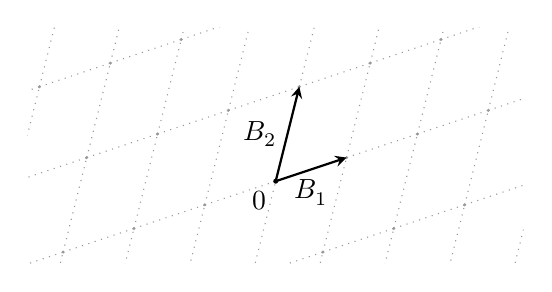
\begin{tikzpicture}[scale=0.3]
        \clip (-10.5, -3.5) rectangle (10.5, 6.5);

        \foreach \x in {-10,...,10}
        \foreach \y in {-10,...,10}
        {
          \draw[black!40, dotted] (3*\x + \y, \x + 4*\y) -- (3*\x + \y + 1, \x + 4*\y + 4);
          \draw[black!40, dotted] (3*\x + \y, \x + 4*\y) -- (3*\x + 3 + \y, \x + 1 + 4*\y);
          \fill[black!40] (3*\x + \y, \x + 4*\y) circle (2pt);
        }

        \draw[->, thick] (0, 0) -- node[below] {$B₁$} (3, 1);
        \draw[->, thick] (0, 0) -- node[left] {$B₂$} (1, 4);
        \fill (0, 0) circle (3pt) node[below left] {$0$};
      \end{tikzpicture}
    \end{center}
  \end{columns}
\end{frame}

\begin{frame}[fragile]
  \frametitle{Modulo}
  \small
  \begin{columns}
    \column{0.49\textwidth}
    \begin{center}
      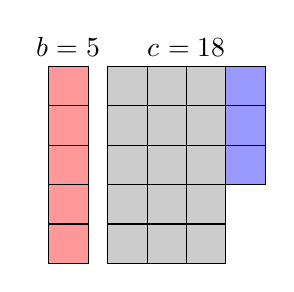
\begin{tikzpicture}[scale=0.5]
  % Parameters
  \def\a{18}     % total number
  \def\b{5}      % divisor
  \pgfmathsetmacro{\q}{int(\a/\b)} % quotient
  \pgfmathsetmacro{\r}{mod(\a,\b)} % remainder

  % Draw squares
  \foreach \i in {0,...,\numexpr\a-1} {
    \pgfmathtruncatemacro{\col}{int(\i/\b)}
    \pgfmathtruncatemacro{\row}{int(mod(\i,\b))}
    \ifnum\col=\q
    \draw[fill=blue!40] (\col, -\row) rectangle ++(1, -1); % remainder
    \else
    \draw[fill=black!20] (\col, -\row) rectangle ++(1, -1); % full blocks
    \fi
  }

  \foreach \i in {0,...,\numexpr\b-1} {
    \draw[fill=red!40] (-1.5, -\i) rectangle ++(1, -1);
  }

  \path (-1.5, 0) -- ++(1, 0) node[midway, above] {$b = \b$};
  \path (0, 0) -- ++(\q+1, 0) node[midway, above] {$c = \a$};
\end{tikzpicture}


    \end{center}
    \[
      c = \symbfit{\color{red}b} \floor{x} + \symbfit{\color{blue}r}
    \]

    \column{0.49\textwidth}
    \adjustbox{scale=0.7}{\includestandalone{figures/lattice-modulo}}
    \[
      c = {\underbrace{B \floor{x}}_{{} ∈ \mathcal L(B)}} + {\underbrace{r}_{{} ∈ Π(B)}}
    \]
  \end{columns}
\end{frame}

\begin{frame}[fragile]
  \frametitle{Exchange}
  \small
  \begin{columns}
    \column{0.49\textwidth}
    \begin{center}
      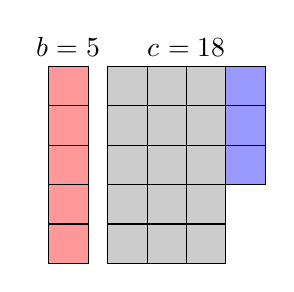
\begin{tikzpicture}[scale=0.5]
  % Parameters
  \def\a{18}     % total number
  \def\b{5}      % divisor
  \pgfmathsetmacro{\q}{int(\a/\b)} % quotient
  \pgfmathsetmacro{\r}{mod(\a,\b)} % remainder

  % Draw squares
  \foreach \i in {0,...,\numexpr\a-1} {
    \pgfmathtruncatemacro{\col}{int(\i/\b)}
    \pgfmathtruncatemacro{\row}{int(mod(\i,\b))}
    \ifnum\col=\q
    \draw[fill=blue!40] (\col, -\row) rectangle ++(1, -1); % remainder
    \else
    \draw[fill=black!20] (\col, -\row) rectangle ++(1, -1); % full blocks
    \fi
  }

  \foreach \i in {0,...,\numexpr\b-1} {
    \draw[fill=red!40] (-1.5, -\i) rectangle ++(1, -1);
  }

  \path (-1.5, 0) -- ++(1, 0) node[midway, above] {$b = \b$};
  \path (0, 0) -- ++(\q+1, 0) node[midway, above] {$c = \a$};
\end{tikzpicture}


      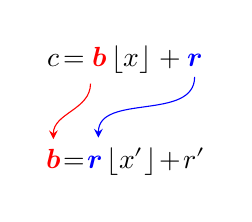
\begin{tikzpicture}
        \node[matrix, matrix of math nodes, column sep=-2mm, row sep=7mm] (M)
        {
          c   & =  & \symbfit{\color{red}b} \floor{x} &+& \symbfit{\color{blue}r} \\
          \symbfit{\color{red}b}   & =  & \symbfit{\color{blue}r} \floor{x'} &+& r' \\
        };

        \draw[->, blue, in=90, out=270] (M-1-5.south) to ([xshift=-3mm]M-2-3.north);
        \draw[->, red, in=90, out=270] ([xshift=-4mm]M-1-3.south) to (M-2-1);
      \end{tikzpicture}
    \end{center}

    \column{0.49\textwidth}
    \adjustbox{scale=0.7}{\includestandalone{figures/lattice-modulo}}
    \begin{center}
      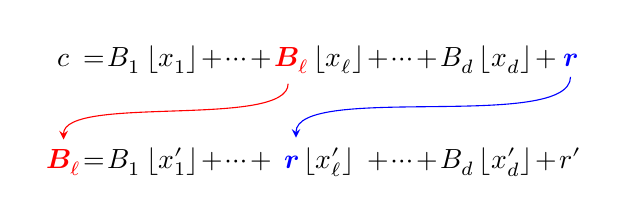
\begin{tikzpicture}
        \node[matrix, matrix of math nodes, column sep=-2mm, row sep=7mm] (M)
        {
          c   & =  & B_1 \floor{x_1}  & + & ⋯ & + & \symbfit{\color{red}B_ℓ} \floor{x_ℓ} & + & ⋯ & + & B_d \floor{x_d}   & + & \symbfit{\color{blue}r}   \\
          \symbfit{\color{red}B_ℓ} & =  & B_1 \floor{x_1'} & + & ⋯ & + & \symbfit{\color{blue}r} \floor{x_ℓ'}  & + & ⋯ & + & B_d \floor{x_d'}  & + & r'  \\
        };

        \draw[->, blue, in=90, out=270, looseness=0.5] (M-1-13.south) to ([xshift=-3mm]M-2-7.north);
        \draw[->, red, in=90, out=270, looseness=0.5] ([xshift=-4mm]M-1-7.south) to (M-2-1);
      \end{tikzpicture}
    \end{center}
  \end{columns}
\end{frame}

\begin{frame}
  \frametitle{Fibonacci Numbers}
  \small
  \begin{columns}[T]
    \column{0.49\textwidth}
    The Fibonacci numbers are defined as
    \[
      F(n) = F(n - 1) + F(n - 2).
    \]
    \column{0.49\textwidth}
    The $d$-bonacci numbers are defined as
    \[
      F_d(n) = F_d(n - 1) + ⋯ + F_d(n - d - 1).
    \]
  \end{columns}
  \vspace{1em}
  \begin{columns}[T]
    \column{0.49\textwidth}
    \begin{theorem}
      If the Euclidean algorithm requires $n$ steps on $(a, b)$ with $a < b$,
      then \[
        a ≥ F(n+1) \text{ and } b ≥ F(n+2).
      \]
    \end{theorem}

    \column{0.49\textwidth}
    \begin{theorem}
      If the generalized Euclidean algorithm requires $n$ steps on $x = (p₁/q, …, p_d/q)$,
      when selecting the \alert{minimum fractional value},
      then \[
        p_{σ(i)} ≥ ∑_{k=0}^i F_d(n-k) \text{ and } q ≥ F_d(n)
      \]
      for some permutation $σ$.
    \end{theorem}
  \end{columns}
\end{frame}

\begin{frame}
  \frametitle{Golden Ratio}

  \begin{columns}
    \column{0.49\textwidth}
    \begin{center}
      \begin{tikzpicture}[scale=3]
        \def\width{1.6180339}
        \def\height{1}

        \fill[black!30] (0, 0) rectangle (\height, \height);
        \path (0, 0) rectangle (\height, \height) node[midway] {$1:1$};
        \path (\height, 0) rectangle (\width, \height) node[midway, black] {$1:φ^{-1}$};
        \draw (0, 0) rectangle (\width, \height);
        \draw[dashed] (\height, 0) -- (\height, \height) node[above] {\emoji{scissors}};

        \draw[<->] (0, -0.1) -- (\width, -0.1) node[midway, below] {$φ$};
        \draw[<->] (-0.1, 0) -- (-0.1, \height) node[midway, left] {$1$};
      \end{tikzpicture}
    \end{center}
    \[
      \lim_{n → ∞} \frac{F(n+1)}{F(n)} = φ
    \]

    \column{0.49\textwidth}
    \begin{center}
      \begin{tikzpicture}[scale=1.5]
        % Define dimensions
        \def\width{1}         % along y-axis (ψ)
        \def\depth{1.465571}  % along x-axis
        \def\height{1.68232} % along z-axis (ψ²)

        % Define corners of the cuboid
        \coordinate (O) at (0, 0);                            % origin
        \coordinate (A) at (\depth, 0);                      % x
        \coordinate (B) at (\depth, \width);                 % x+y
        \coordinate (C) at (0, \width);                      % y

        \coordinate (O') at (0, 0, \height);                 % origin shifted up
        \coordinate (A') at (\depth, 0, \height);            % x up
        \coordinate (B') at (\depth, \width, \height);       % x+y up
        \coordinate (C') at (0, \width, \height);            % y up

        \fill[black!30] (O') -- (\width, 0, \height) -- (\width, \width, \height) -- (0, \width, \height);
        \path (0, 0, \height) rectangle (\width, \width, \height) node[midway] {$1:1$};
        \fill[black!30] (A) -- (\depth, \width) -- (\depth, \width, \width) -- (\depth, 0, \width);
        \fill[black!30] (0, \width, \height) -- (0, \width) -- (\width, \width) -- (\width, \width, \height);
        \fill[black!30] (B) -- (C) -- (0, \width, \width) -- (\depth, \width, \width);

        \begin{scope}[canvas is zy plane at x=\depth]
          \path (0, 0) rectangle (\width, \width) node[midway, transform shape, xscale=-1, scale=0.8] {$1:1$};
        \end{scope}

        %\fill (O') -- (\width, 0, \height) -- (\width, \width, \height) -- (0, \width, \height);

        % Draw cuboid
        \draw (O') -- (A') -- (B') -- (C') -- cycle;
        \draw (A') -- (A);
        \draw (B') -- (B);
        \draw (C') -- (C);
        \draw (A) -- (B) -- (C);

        % Draw cuts
        \draw[dashed] (\depth, 0, \width) -- (\depth, \width, \width) -- (0, \width, \width) node[rotate=90, above] {\emoji{scissors}};
        \draw[dashed] (\width, 0, \height) -- (\width, \width, \height) -- (\width, \width) node[rotate=-45, above] {\emoji{scissors}};

        % Label dimensions
        \draw[<->] (\depth + 0.2, 0) -- (\depth + 0.2, \width) node[midway, right] {$1$};
        \draw[<->] (0, -0.2, \height) -- (\depth, -0.2, \height) node[midway, below] {$φ_d$};
        \draw[<->] (\depth, -0.2, 0) -- (\depth, -0.2, \height) node[midway, below right] {$φ_d^2 - φ_d$};
      \end{tikzpicture}
    \end{center}
    \[
      \lim_{n → ∞} \frac{F_d(n+1)}{F_d(n)} = φ_d
    \]
  \end{columns}
\end{frame}

\begin{frame}<1>[label={cont-frac}]
  \frametitle{Continued Fractions}
  \small
  \begin{columns}[T]
    \column{0.49\textwidth}
    \begin{definition}
      A \emph{continued fraction} over a sequence over integers $(aₙ)_{n≥0}$ is defined as
      \[
        [a₀; a₁, …] = a₀ + \frac{1}{[a₁; a₂, …]}.
      \]
      The \emph{$n$-th convergent} is $[a₀; a₁, …, aₙ]$.
    \end{definition}

    \pause
    \column{0.49\textwidth}
    \begin{definition}
      A \emph{multidimensional continued fraction} over a sequence over integer
      vectors $(a^{(n)})_{n≥0}$ is defined as
      \[
        [a^{(0)}; a^{(1)}, …] = \mathrm{pivot}^{-1}(a^{(0)}, [a^{(1)}; a^{(2)}, …]).
      \]
      The \emph{$n$-th convergent} is $[a^{(0)}; a^{(1)}, …, a^{(n)}]$.
    \end{definition}
  \end{columns}
\end{frame}

\begin{frame}[fragile]
  \frametitle{Construction}

  \begin{columns}
    \column{0.49\textwidth}
    \begin{center}
      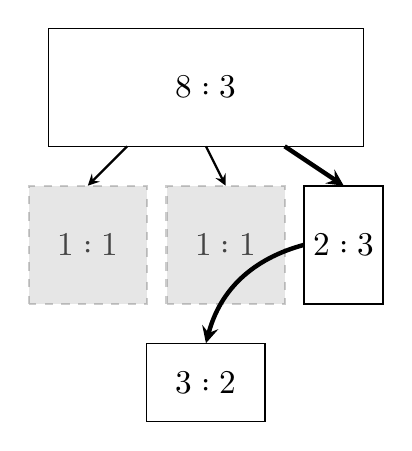
\begin{tikzpicture}[scale=0.5]
        \draw (0, 0) rectangle (8, 3) node[pos=0.5] {\large $8:3$};

        \draw[thick, dashed, fill=black!50, opacity=0.2] (-0.5, -4) rectangle (2.5, -1) node[pos=0.5, opacity=0.7] {\large$1:1$};
        \draw[thick, dashed, fill=black!50, opacity=0.2] (3, -4) rectangle (6, -1) node[pos=0.5, opacity=0.7] {\large$1:1$};
        \draw[thick] (6.5, -4) rectangle (8.5, -1) node[pos=0.5] {\large$2:3$};

        \draw (2.5, -7) rectangle (5.5, -5) node[pos=0.5] {\large$3:2$};

        \draw[ultra thick] (6.5, -2.5) edge[bend right, ->] (4, -5);
        \draw[thick] (2, 0) edge[->] (1, -1);
        \draw[thick] (4, 0) edge[->] (4.5, -1);
        \draw[ultra thick] (6, 0) edge[->] (7.5, -1);
      \end{tikzpicture}
    \end{center}
    \[
      x' = \frac{1}{x - \lfloor{x}\rfloor}
    \]

    \column{0.49\textwidth}
    \begin{center}
      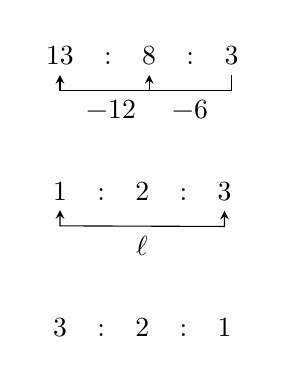
\begin{tikzpicture}
        \matrix[matrix of nodes, column sep=1ex] (m)
        {
          \node (a) {13}; & \node{:}; &
          \node (b) {8};  & \node{:}; &
          \node (c) {3}; \\
        };

        \matrix[matrix of nodes, column sep=1ex, below=of m] (m2)
        {
          \node (a2) {1}; & \node{:}; &
          \node (b2) {2};  & \node{:}; &
          \node (c2) {3}; \\
        };


        \matrix[matrix of nodes, column sep=1ex, below=of m2] (m3)
        {
          \node (a3) {3}; & \node{:}; &
          \node (b3) {2};  & \node{:}; &
          \node (c3) {1}; \\
        };

        \draw[->] (c) -- ($(c.south)-(0,0.2)$) -- ($(a.south)-(0,0.2)$) node[pos=0.7, below] {$-12$} -- (a);
        \draw[->] (c) -- ($(c.south)-(0,0.2)$) -- ($(b.south)-(0,0.2)$) node[pos=0.5, below] {$-6$} -- (b);

        \draw[<->] (c2) -- ($(c2.south)-(0,0.2)$) -- ($(a2.south)-(0,0.2)$) node[midway, below] {$ℓ$} -- (a2);
      \end{tikzpicture}
    \end{center}
    \begin{align*}
      x' & = \mathrm{pivot}_ℓ(x) \\
      \text{ with } x_i' & =
      \begin{cases}
        \frac{1}{x_ℓ - a_ℓ}, & \text{ if } i = ℓ, \\
        \frac{x_i - \floor{x_i}}{x_ℓ - \floor{x_ℓ}}, & \text{ otherwise}.
      \end{cases}
    \end{align*}
  \end{columns}
\end{frame}

\begin{frame}
  % TODO: Figure for pivot rule
  \[
    x' = \mathrm{pivot}_ℓ(x)
    \iff
    x = \mathrm{pivot}^{-1}(a, x').
  \]
  \[
    x_i' =
    \begin{cases}
      \frac{1}{x_ℓ - a_ℓ}, & \text{ if } i = ℓ, \\
      \frac{x_i - a_i}{x_ℓ - a_ℓ}, & \text{ otherwise},
    \end{cases}
    \iff
    x_i =
    \begin{cases}
      a_ℓ + \frac{1}{x_ℓ'}, & \text{ if } i = ℓ, \\
      a_i + \frac{x_i'}{x_ℓ'}, & \text{ otherwise}.
    \end{cases}
  \]
\end{frame}

\againframe<2>{cont-frac}

\begin{frame}
  \frametitle{Convergence}
  \small
  \begin{columns}
    \column{0.49\textwidth}
    \begin{onlyenv}<1>
      \begin{theorem}
        The convergents $pₙ/qₙ$ of a continued fraction approach $x ∈ ℝ$.
        Specifically,
        \[
          \left|x - \frac{pₙ}{qₙ}\right| < \frac{1}{qₙ^2}.
        \]
      \end{theorem}
    \end{onlyenv}
    \begin{onlyenv}<2>
      \adjustbox{scale=1}{\includestandalone{figures/convergence}}
    \end{onlyenv}

    \column{0.49\textwidth}
    \begin{theorem}
      The convergents $r^{(n)}$ of a multidimensional continued fraction approach $x ∈ ℝ^d$, if
      \begin{enumerate}
        \item Every index is used infinitely often
        \item The distance between two equal indices is constant.
      \end{enumerate}
    \end{theorem}
  \end{columns}
\end{frame}

\begin{frame}
  \frametitle{Geometry}
  \small

  \begin{columns}[T]
    \column{0.41\textwidth}
    The \emph{$n$-th convergent} is $[a₀; a₁, …, aₙ]$.
    \begin{lemma}
      \begin{onlyenv}<1>
        \[
          \frac{pₙ}{qₙ} = \frac{p_{n-1} a_n + p_{n-2}}{q_{n-1} a_n + q_{n-2}}.
        \]
        \vspace{8em}
      \end{onlyenv}
      \begin{onlyenv}<2>
        \begin{align*}
          \binom{p_n}{q_n}
          & = \begin{pmatrix}
            p_{n-1} \\ q_{n-1} \\
          \end{pmatrix} a_n + \begin{pmatrix}
            p_{n-2} \\ q_{n-2} \\
          \end{pmatrix} \\
          & = \begin{pmatrix}
            p_{n-1} & p_{n-2} \\
            q_{n-1} & q_{n-2} \\
          \end{pmatrix}
          \begin{pmatrix}
            a_n \\
            1 \\
          \end{pmatrix} \\
          & =
          B_n
          \begin{pmatrix}
            a_n \\
            1 \\
          \end{pmatrix}.
        \end{align*}
      \end{onlyenv}
    \end{lemma}

    \column{0.61\textwidth}
    The \emph{$n$-th convergent} is $[a^{(0)}; a^{(1)}, …, a^{(n)}]$.
    \begin{lemma}
      \begin{onlyenv}<1>
        \[
          \frac{P_ℓ^{(n)}}{Q_ℓ}
          = \frac{P_0^{(n-1)} + P_1^{(n-1)} a_1^{(n)} + ⋯ + P_d^{(n)} a_d^{(n)}}
                 {Q_0^{(n-1)} + Q_1^{(n-1)} a_1^{(n)} + ⋯ + Q_d^{(n)} a_d^{(n)}}.
        \]
      \end{onlyenv}
      \begin{onlyenv}<2>
        \begin{align*}
          \begin{pmatrix}
            P_ℓ^{(n)} \\
            Q_ℓ^{(n)} \\
          \end{pmatrix}
          & = \begin{pmatrix}
            P_0^{(n-1)} \\
            Q_0^{(n-1)} \\
          \end{pmatrix} +
          \begin{pmatrix}
            P_1^{(n-1)} \\
            Q_1^{(n-1)} \\
          \end{pmatrix} a_1^{(n)} + ⋯ +
          \begin{pmatrix}
            P_1^{(n-1)} \\
            Q_1^{(n-1)} \\
          \end{pmatrix} a_d^{(n)} \\
          & = \begin{pmatrix}
            P_0^{(n-1)} & P_1^{(n-1)} & ⋯ & P_d^{(n-1)} \\
            Q_0^{(n-1)} & Q_1^{(n-1)} & ⋯ & Q_d^{(n-1)} \\
          \end{pmatrix}
          \begin{pmatrix}
            a^{(n)} \\
            1 \\
          \end{pmatrix} \\
          & = B^{(n)}
          \begin{pmatrix}
            a^{(n)} \\
            1 \\
          \end{pmatrix}.
        \end{align*}
      \end{onlyenv}
    \end{lemma}
  \end{columns}
\end{frame}

\begin{frame}
  \begin{columns}
    \column{0.49\textwidth}
    \includestandalone{figures/klein-polygon}

    \column{0.49\textwidth}
    \includestandalone{figures/projective-space}
  \end{columns}
\end{frame}

\begin{frame}
  \frametitle{Periodicity $\Rightarrow$ Algebraicity}
  \footnotesize
  \begin{columns}[T]
    \column{0.49\textwidth}
    \begin{theorem}
      If a continued fraction of a number $x ∈ ℝ$ is periodic, then $x$ is a
      quadratic irrational.
    \end{theorem}

    \begin{proof}[Proof Sketch]
      If the continued fraction is periodic,
      then
      \[
        B_{n+k} \binom{x_n}{1} = λ \binom{x_n}{1}. \qedhere
      \]
    \end{proof}

    \column{0.49\textwidth}
    \begin{theorem}
      If a multidimensional continued fraction of a vector $x ∈ ℝ^d$ is
      periodic, then $[ℚ(x₁, …, x_d) : ℚ] ≤ d+1$.
    \end{theorem}

    \begin{proof}[Proof Sketch]
      If the multidimensional continued fraction is eventually periodic, then
      \[
        B^{(n+k)} \binom{x^{(n)}}{1} = λ \binom{x^{(n)}}{1}. \qedhere
      \]
    \end{proof}
  \end{columns}
\end{frame}

\begin{frame}
  \frametitle{Periodicity $\Leftarrow$ Algebraicity?}
  \small
  \begin{columns}
    \column{0.49\textwidth}
    \begin{theorem}
      If $x$ is a quadratic irrational,
      then its continued fraction is periodic.
    \end{theorem}

    \begin{proof}[Proof Sketch]
      For every quadratic irrational,
      there exists a matrix $U ∈ ℤ^{2×2}$, which preserves the Klein polygon and thus, the convergents.
    \end{proof}

    \column{0.49\textwidth}
    \begin{onlyenv}<1>
      \begin{conjecture}
        If $x$ is an algebraic number of degree $d+1$,
        then the multidimensional continued fraction of $(x^1, …, x^d)$ is
        periodic.
      \end{conjecture}

      \begin{itemize}
        \item[$\Rightarrow$] There are periodic MCFs up to $\sqrt[3]{10\,000}$.
        \item[$\Rightarrow$] There are periodic MCFs up to $\sqrt[4]{10\,000}$.
      \end{itemize}
    \end{onlyenv}
    \begin{onlyenv}<2>
      \adjustbox{scale=0.9}{\includestandalone{figures/klein-polygon}}
    \end{onlyenv}
    \begin{onlyenv}<3>
      \adjustbox{scale=0.7}{\includestandalone{figures/full-klein-polygon}}
    \end{onlyenv}
  \end{columns}
\end{frame}

\begin{frame}
  \small
  \begin{columns}
    \column{0.49\textwidth}
    \begin{enumerate}
      \item The Euclidean Algorithm
      \item Fibonacci Numbers
      \item Continued Fractions
      \item Periodicity and Quadratic Irrationals
    \end{enumerate}

    \column{0.49\textwidth}
    \begin{enumerate}
      \item The Generalized Euclidean Algorithm
      \item Higher-Order Fibonacci Numbers
      \item Multidimensional Continued Fractions
      \item Periodicity and Algebraic Numbers?
    \end{enumerate}
  \end{columns}
\end{frame}

\begin{frame}

\end{frame}

\end{document}
